\addcontentsline{toc}{chapter}{Занятие 2. Характеристики случайного процесса}
\chapter*{Занятие 2. Характеристики случайного процесса}

\addcontentsline{toc}{section}{Контрольные вопросы и задания}
\section*{Контрольные вопросы и задания}

\subsubsection*{Приведите определение случайного процесса.}

Случайный процесс $ \xi \left( t \right), \, t \in T$ ---
это параметризированная совокупность случайных величин.

\subsubsection*{Что называют конечномерными распределениями случайного процесса?}

$ \left\{ \mu_{t_1, \dotsc, t_n}; \, t_1, \dotsc, t_n \in T, \, n \geq 1 \right\} $ ---
набор конечномерных распределений процесса $ \xi $, где $ \mu_{t_1, \dotsc, t_n}$ ---
распределение вектора $ \left( \xi \left( t_1 \right), \dotsc, \xi \left( t_n \right) \right) $ в
$ \mathbb{R}^n$,
то есть для борелевского
$ \Delta \in \mathcal{B} \left( \mathbb{R}^n \right), \,
  \mu_{t_1, \dotsc, t_n} \left( \Delta \right) =
  P \left\{
    \left( \xi \left( t_1 \right), \dotsc, \xi \left( t_n \right) \right) \in \Delta
  \right\} $.

\subsubsection*{Приведите определение функции математического ожидания,
                дисперсии и ковариационной функции случайного процесса.}

$m \left( t \right) = M \xi \left( t \right), \, t \in T$ --- функция среднего.

$D \xi \left( t \right), \, t \in T$ --- функция дисперсии.

$K \left( t, s \right) =
  M \left[ \xi \left( t \right) - m \left( t \right) \right] \cdot
  \left[ \xi \left( s \right) - m \left( s \right) \right], \, t, s \in T$ ---
функция ковариации.

\addcontentsline{toc}{section}{Аудиторные задачи}
\section*{Аудиторные задачи}

\subsubsection*{2.2}

\textit{Задание.}
Пусть
$$ \xi \left( t \right) =
  X \cdot e^{-t}, \,
  t > 0,$$
где $X$ --- случайная величина,
которая имеет нормальное распределение с параметрами $a, \, \sigma^2$.
Найдите математическое ожидание, дисперсию,
ковариационную функцию и одномерную плотность распределения случайного процесса
$ \xi =
  \left\{ \xi \left( t \right), \, t > 0 \right\} $.

\textit{Решение.}
Сейчас $T = \left( 0, \infty \right) $.

Случайная величина $X$ имеет распределение $N \left( a, \sigma^2 \right) $.
Нужно найти $M \xi \left( t \right) = m \left( t \right), \, D \xi \left( t \right) $,
ковариационную функцию $K \left( t, s \right) $ и одномерную плотность распределения
$p_{ \xi } \left( t \right) $.

Найчнём с математического ожидания
$$m \left( t \right) =
  M \left( X \cdot e^{-t} \right) =
  e^{-t} MX =
  e^{-t} \cdot a.$$

Далее ---
функция дисперсии $D \xi \left( t \right) = D \left( X \cdot e^{-t} \right) = e^{-2t} \cdot DX$.
Дисперсия $X$ --- известная: $e^{-2t} \cdot DX = e^{-2t} \cdot \sigma^2$.

Далее ---
ковариационная функция
$$K \left( t, s \right) =
  M \left[ \xi \left( t \right) - m \left( t \right) \right] \cdot
  \left[ \xi \left( s \right) - m \left( s \right) \right] =
  cov \left[ \xi \left( t \right), \xi \left( s \right) \right].$$
Вместо $ \xi \left( t \right), \, \xi \left( s \right) $ подставляем их значения
$$cov \left[ \xi \left( t \right), \xi \left( s \right) \right] =
  cov \left( Xe^{-t}, Xe^{-s} \right).$$
Множители выносятся
$$cov \left( Xe^{-t}, Xe^{-s} \right) =
  e^{-t - s} cov \left( X, X \right) =
  e^{-t - s} DX =
  e^{-t - s} \sigma^2.$$

Последнее ---
это плотность $ \xi \left( t \right) \sim N \left( e^{-t} a, \, e^{-2t} \sigma^2 \right) $.

Нужно написать нормальную плотность с заданными математическим ожиданием и дисперсией
$$p_{ \xi \left( t \right) } \left( x \right) =
  \frac{1}{ \sqrt{2 \pi e^{-2t} \sigma^2}} \cdot
  e^{- \frac{ \left( x - e^{-t} a \right)^2}{2e^{-2t} \sigma^2}}.$$

Траектория процесса изображена на рисунке \ref{fig:22}
и имеет разный вид в зависимости от значения случайной величины $X$.

\begin{figure}[h!]
  \centering
  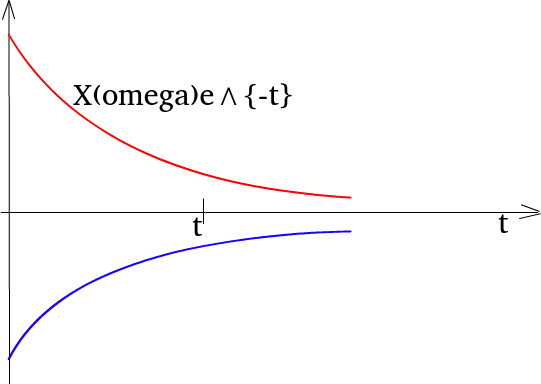
\includegraphics[width=.4\textwidth]{./pictures/2_2.png}
  \caption{Траектория процесса}
  \label{fig:22}
\end{figure}

\subsubsection*{2.3}

\textit{Задание.}
Пусть
$$ \xi \left( t \right) =
  e^{-Xt}, \,
  t > 0,$$
где $X$ --- случайная величина, которая имеет показательное распределение с параметром $ \lambda $.
Запишите конечномерные распределения случайного процесса
$ \left\{ \xi \left( t \right), \, t > 0 \right\} $.
Найдите его математическое ожидание, дисперсию и ковариационную функцию.

\textit{Решение.}
$ \xi \left( t \right) = e^{-Xt}$, где $X \sim Exp \left( \lambda \right), \, t > 0$.

Нужно найти $m \left( t \right), \, K \left( t, s \right) $, конечномерные распределения.

Найдём математическое ожидание в момент $t$.
По определению
$$m \left( t \right) =
  Me^{-Xt} =
  \int \limits_0^{+ \infty } \lambda e^{- \lambda x} e^{-Xt} dX =
  \frac{ \lambda }{ \lambda + t}.$$
Траектории такого процесса изображены на рисунке \ref{fig:23}: чем больше $X$,
тем быстрее эта функция убывает.

\begin{figure}[h!]
  \centering
  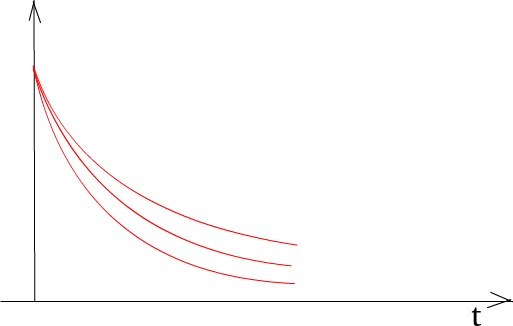
\includegraphics[width=.4\textwidth]{./pictures/2_3.png}
  \caption{Траектория процесса}
  \label{fig:23}
\end{figure}

Ковариационная функция считается по определению
$$K \left( t, s \right) =
  M \xi \left( t \right) \xi \left( s \right) - M \xi \left( t \right) M \xi \left( s \right) =
  Me^{-Xt - Xs} - \frac{ \lambda }{ \lambda + t} \cdot \frac{ \lambda }{ \lambda + s}.$$
Подставим найденное значение фунцкии математического ожидания
$$Me^{-Xt - Xs} - \frac{ \lambda }{ \lambda + t} \cdot \frac{ \lambda }{ \lambda + s} =
  \frac{ \lambda }{ \lambda + t + s} -
  \frac{ \lambda^2}{ \left( \lambda + t \right) \left( \lambda + s \right) }.$$

Считаем функцию распределения случайного вектора
$ \left( \xi \left( t_1 \right), \dotsc, \xi \left( t_n \right) \right) $ --- рис. \ref{fig:231}.

\begin{figure}[h!]
  \centering
  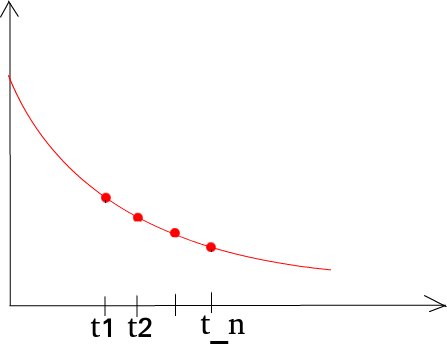
\includegraphics[width=.4\textwidth]{./pictures/2_3_1.png}
  \caption{Выбираем точки, в которых ищем распределение случайного процесса}
  \label{fig:231}
\end{figure}

$F_{ \left( \xi \left( t_1 \right), \dotsc, \xi \left( t_n \right) \right) }
  \left( \vec{x} \right) =
  P \left\{ \xi \left( t_1 \right) \leq x_1, \dotsc, \xi \left( t_n \right) \leq x_n \right\} $.
Вместо $ \xi $ напишем формулу
$P \left\{ \xi \left( t_1 \right) \leq x_1, \dotsc, \xi \left( t_n \right) \leq x_n \right\} =
  P \left( e^{-Xt_1} \leq x_1, \dotsc, e^{-Xt_n} \leq x_n \right) $.
Величины зависимы, потому что все они выражаются через $X$.
Все неравенства решаем относительно $X$
$$P \left( e^{-Xt_1} \leq x_1, \dotsc, e^{-Xt_n} \leq x_n \right) =
  P \left\{ X \geq -\frac{ln \, x_1}{t_1}, \dotsc, X \geq -\frac{ln \, x_n}{t_n} \right\}.$$
Перепишем через максимум
$$P \left\{ X \geq -\frac{ln \, x_1}{t_1}, \dotsc, X \geq -\frac{ln \, x_n}{t_n} \right\} =
  P \left\{
    X \geq \max \left( -\frac{ln \, x_1}{t_1}, \dotsc, -\frac{ln \, x_n}{t_n} \right) \right\}.$$
Обозначим максимум буквой $m$
$$P \left\{
    x \geq \max \left( -\frac{ln \, x_1}{t_1}, \dotsc, -\frac{ln \, x_n}{t_n} \right) \right\} =
  \int \limits_m^{+\infty } \lambda e^{-\lambda X} dX =
  -\left. e^{-\lambda X} \right|_m^{+\infty}.$$
На бесконечности получаем ноль
$$-\left. e^{-\lambda X} \right|_m^{+\infty} =
  e^{-\lambda m} =
  e^{-\lambda \max \left( ln \, x_1^{-\frac{1}{t_1}}, \dotsc, ln \, x_n^{-\frac{1}{t_n}} \right) }.$$
Выносим логарифм
$$e^{-\lambda \max \left( ln \, x_1^{-\frac{1}{t_1}}, \dotsc, ln \, x_n^{-\frac{1}{t_n}} \right) } =
e^{-\lambda ln \max \left( x_1^{-\frac{1}{t_1}}, \dotsc, x_n^{-\frac{1}{t_n}} \right) }.$$
Экспонента и логарифм уничтожают друг друга
$$e^{-\lambda ln \max \left( x_1^{-\frac{1}{t_1}}, \dotsc, x_n^{-\frac{1}{t_n}} \right) } =
  \max \left( x_1^{-\frac{1}{t_1}}, \dotsc, x_n^{-\frac{1}{t_n}} \right)^{-\lambda } =
  \min \left( x_1^{ \frac{ \lambda }{t_1}}, \dotsc, x_n^{ \frac{ \lambda }{t_n}} \right).$$

Все выкладки были законные, только когда $0 < x_1, \dotsc, x_n < 1$.

Плотности у такого векора $ \left( \xi \left( t_1 \right), \dotsc, \xi \left( t_n \right) \right) $
быть не может, потому что
$ \xi \left( t_1 \right)^{ \frac{1}{t_1}} =
  e^{-X} =
  \xi \left( t_2 \right)^{ \frac{1}{t_2}}$.
Сейчас у нас только одна случайная величина.
Это можно переписать как
$ \xi \left( t_2 \right) = \xi \left( t_1 \right)^{ \frac{t_2}{t_1}}, \,
  y = x^{ \frac{t_2}{t_1}}.$

С вероятностью 1 $ \left( \xi \left( t_1 \right), \xi \left( t_2 \right) \right) \in L$ ---
рис. \ref{fig:232}.

\begin{figure}[h!]
  \centering
  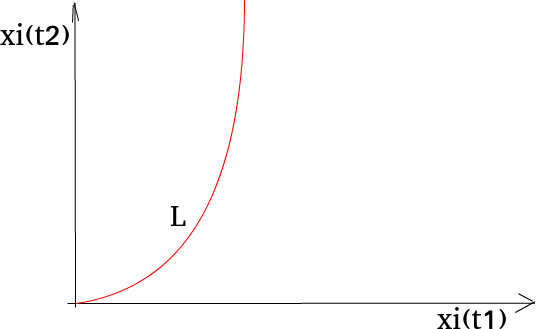
\includegraphics[width=.5\textwidth]{./pictures/2_3_2.png}
  \caption{$y = x^{ \frac{t_2}{t_1}}$}
  \label{fig:232}
\end{figure}

Значения вектора всегда попадают на такую линию.
Площадь кривой --- ноль.

Плотность --- производная от функции распределения, а минимум нельзя дифференцировать.

\subsubsection*{2.4}

\textit{Задание.}
Рассмотрим случайный процесс
$$X \left( t \right) =
  A \cos \left( \varphi + \lambda t \right),$$
где $A$ и $ \varphi $ являются независимыми случайными величинами такими, что $MA^2 < \infty $,
а $ \varphi $ имеет равномерное распределение на отрезке $ \left[ 0, 2 \pi \right] $.
Найдите математическое ожидание и ковариационную функцию процесса
$$ \left\{ X \left( t \right), \, t \geq 0 \right\}.$$

\textit{Решение.} $ \varphi \sim U \left( \left[ 0, 2 \pi \right] \right) $.

Траектория такого процесса изображена на рисунке \ref{24}.

\begin{figure}[h!]
 \centering
 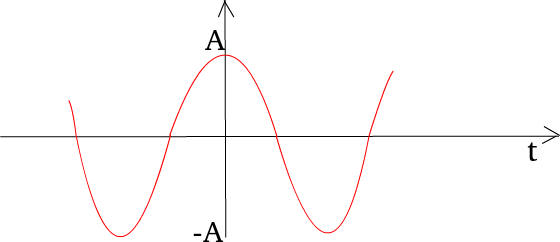
\includegraphics[width=.5\textwidth]{./pictures/2_4.png}
 \caption{Траектория процесса}
 \label{fig:24}
\end{figure}

Тут случайная амплитуда и случайный сдвиг по фазе.

$MX \left( t \right) =
M \left[ A \cos \left( \varphi + \lambda t \right) \right] $.
Случайные величины $A$ и $ \varphi $ --- независимые.
$M \left[ A \cos \left( \varphi + \lambda t \right) \right] =
  MAM \cos \left( \varphi + \lambda t \right) $.
Математическое ожидание косинуса можем найти, потому что у $ \varphi $ известна плотность
$$MAM \cos \left( \varphi + \lambda t \right) =
  MA \cdot \int \limits_0^{2 \pi }
    \cos \left( \varphi + \lambda t \right) \cdot \frac{1}{2 \pi } \cdot d \varphi.$$
Интеграл косинуса по периоду --- ноль.

Ковариационная функция
$K \left( t, s \right) =
  MX \left( t \right) X \left( s \right) - MX \left( t \right) MX \left( s \right) =$
Произведение математических ожиданий мы знаем
$$= MX \left( t \right) X \left( s \right) =
  M \left[
    A^2 \cos \left( \varphi + \lambda t \right) \cos \left( \varphi + \lambda s \right) \right] =$$
Используем независимость
$$= MA^2 \cdot
  M \left[ \cos \left( \varphi + \lambda t \right) \left( \varphi + \lambda s \right) \right] =$$
Применяем формулу для произведения косинусов
$$= MA^2 \cdot M \left\{
    \frac{1}{2} \cdot \cos \left[ 2 \varphi + \lambda \left( t + s \right) \right] +
    \frac{1}{2} \cdot \cos \left[ \lambda \left( t - s \right) \right] \right\} =$$
Математическое ожидание первого слагаемого --- ноль
$$= \frac{1}{2} \cdot MA^2 \cdot \cos \left[ \lambda \left( t - s \right) \right].$$

Двумерная характеристика процесса зависит только от расстояния между двумя точками.
Это стационарный процесс.
Его характеристики не меняются при сдвиге.

\subsubsection*{2.5}

\textit{Задание.}
Пусть $ \tau $ --- случайная величина,
которая имеет равномерное распределение на отрезке $ \left[ 0, 1 \right] $,
и пусть $ \left\{ X \left( t \right), \, t \in \left[ 0, 1 \right] \right\} $ --- процесс ожидания,
связанный с этой случайной величиной, то есть
$$X \left( t \right) =
  \mathbbm{1} \left\{ t \geq \tau \right\}, \,
  t \in \left[ 0, 1 \right].$$
Запишите конечномерные распределения процесса
$ \left\{ X \left( t \right), \, t \in \left[ 0, 1 \right] \right\} $,
найдите его математическое ожидание и ковариационную функцию.

\textit{Решение.}
$ \tau $ --- случайная величина с распределением $U \left( \left[ 0 , 1 \right] \right) $.

Сначала нарисуем траекторию такого процесса (рис. \ref{fig:25}).
Случайное $ \tau $ выпало.

\begin{figure}[h!]
 \centering
 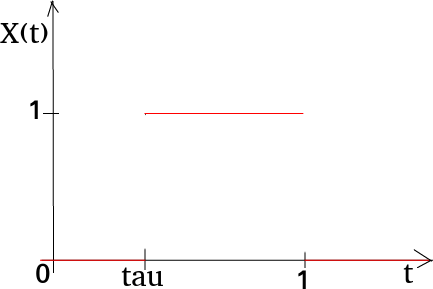
\includegraphics[width=.5\textwidth]{./pictures/2_5.png}
 \caption{Траектория процесса}
 \label{fig:25}
\end{figure}

$$m \left( t \right) =
  MX \left( t \right) =
  M \mathbbm{1} \left\{ t \geq \tau \right\} =
  P \left( t \geq \tau \right) =
  F_{ \tau } \left( t \right) =
  \frac{t - a}{b - a} =
  t.$$

Ковариационная функция
$K \left( t, s \right) =
  M \left[ X \left( t \right) X \left( s \right) \right] -
  MX \left( t \right) MX \left( s \right) $.
Произведение индикаторов --- это индикатор пересечения
$$M \left[ X \left( t \right) X \left( s \right) \right] -
  MX \left( t \right) MX \left( s \right) =
  P \left\{ \tau \leq \min \left( t, s \right) \right\} - ts =
  \min \left( t, s \right) - t \cdot s.$$

Конечномерные распределения ---
распределение вектора $ \left( X \left( t_1 \right), \dotsc, X \left( t_n \right) \right) $.
Каждый $X$ --- это 0 или 1.
$$P \left\{
    \left( X \left( t_1 \right), \dotsc, X \left( t_n \right) \right) = \left( 0, \dotsc, 0 \right)
  \right\} =
  P \left\{ \tau \in \left( t_n , 1 \right] \right\} =
  1 - t_n.$$
Точки $t_n$ изображены на рисунке \ref{fig:251}.

\begin{figure}[h!]
 \centering
 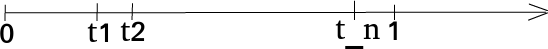
\includegraphics[width=.5\textwidth]{./pictures/2_5_1.png}
 \caption{Временная ось}
 \label{fig:251}
\end{figure}

У вектора получается $ \left( n + 1 \right) $-но значение
$$ \left( X \left( t_1 \right), \dotsc, X \left( t_n \right) \right) =
  \begin{cases}
    \left( 0, \dotsc, 0 \right), \qquad 1 - t_n, \\
    \left( 0, \dotsc, 0, 1 \right), \qquad t_n - t_{n - 1}, \\
    \dotsc, \\
    \left( 0, \dotsc, 0, 1, \dotsc, 1 \right), \qquad t_{k + 1} - t_k, \\
    \dotsc, \\
    \left( 1, \dotsc, 1 \right), \qquad t_1.
  \end{cases}$$

\subsubsection*{2.6}

\textit{Задание.}
Пусть $ \xi_1, \xi_2, \dotsc, \xi_n$ ---
независимые одинаково распределённые случайные величины с функцией распределения $F$, и пусть
$$X \left( t \right) \equiv
  F_n^* \left( t \right) =
  \frac{1}{n} \sum \limits_{i = 1}^n \mathbbm{1} \left\{ \xi_i \leq t \right\}, \,
  t \in \mathbb{R}.$$
Запишите конечномерные распределения процесса
$ \left\{ X \left( t \right), \, t \in \mathbb{R} \right\} $,
найдите его математическое ожидание и ковариационную функцию.

\textit{Решение.}
$$X \left( t \right) =
  \frac{1}{n} \sum \limits_{i = 1}^n \mathbbm{1} \left\{ \xi_i \leq t \right\} $$
--- это эмпирическая функция распределения (рис. \ref{fig:26}).

\begin{figure}[h!]
 \centering
 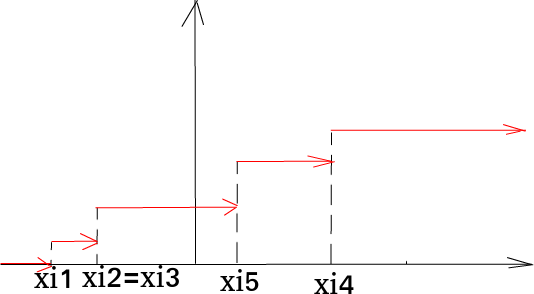
\includegraphics[width=.5\textwidth]{./pictures/2_6.png}
 \caption{Эмпирическая функция распределения}
 \label{fig:26}
\end{figure}

Эмпирическая функция распределения --- это несмещённая оценка функции распределения.

$$cov \left( X \left( t \right), X \left( s \right) \right) =
  cov \left(
    \frac{1}{n} \sum \limits_{i = 1}^n \mathbbm{1} \left\{ \xi_i \leq t \right\}, \,
    \frac{1}{n} \sum \limits_{i = 1}^n \mathbbm{1} \left\{ \xi_i \leq s \right\} \right) =$$
Нужно вынести константы
$$= \frac{1}{n^2}
  \sum \limits_{i,j=1}^n
    cov \left(
      \mathbbm{1} \left\{ \xi_i \leq t, \, \mathbbm{1} \left\{ \xi_j \leq s \right\} \right\}
    \right) =$$
Случайные величины $ \xi_1, \dotsc, \xi_n$ --- независимые.
Ковариация независимых величин --- ноль
$$= \frac{1}{n^2}
  \sum \limits_{i = 1}^n
    \left(
      \mathbbm{1} \left\{ \xi_i \leq t \right\}, \, \mathbbm{1} \left\{ \xi_i \leq s \right\}
    \right).$$

Посчитаем ковариацию двух индикаторов
$$cov \left(
    \mathbbm{1} \left\{ \xi_i \leq t \right\}, \, \mathbbm{1} \left\{ \xi_i \leq s \right\}
  \right) =
  M \mathbbm{1} \left\{ \xi_i \leq t \wedge s \right\} - F \left( t \right) F \left( s \right) =$$
Математическое ожидание индикатора событие --- вероятность этого события,
которая в данном случае по определению равна функции распределения
$$= F \left( t \wedge s \right) - F \left( t \right) F \left( s \right),$$
где $ \wedge $ означает минимум.

Все слагаемые в сумме раны этому выражению
$$K \left( t, s \right) =
  \frac{1}{n} \left[ F \left( t \wedge s \right) - F \left( t \right) F \left( s \right) \right].$$

Теперь нужно написать конечномерные распределения этого процесса.
Фиксируем $t_1, t_2, \dotsc, t_m$ (рис. \ref{fig:261}).

$$X \left( t \right) \in
  \left\{ 0, \frac{1}{n}, \frac{2}{n}, \dotsc, 1 \right\}.$$

По $t, \, X$ увеличивается.
Эта функция монотонна.

\begin{figure}[h!]
 \centering
 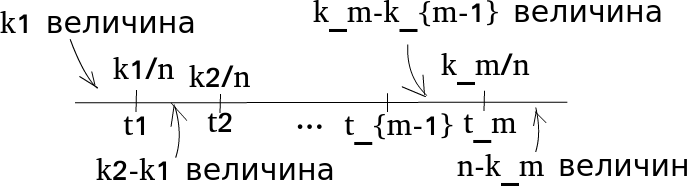
\includegraphics[width=.5\textwidth]{./pictures/2_6_1.png}
 \caption{Фиксируем моменты времени}
 \label{fig:261}
\end{figure}

$0 \leq k_1 \leq k_2 \leq \dotsc \leq k_m \leq n$.

Конечномерные распределения имеют вид
$$P \left\{
    X \left( t_1 \right) = \frac{k_1}{n}, \,
    X \left( t_2 \right) = \frac{k_2}{n}, \dotsc, X \left( t_m \right) = \frac{k_m}{n} \right\} =$$
$P$(для $k_1$ наблюдений $ \xi \leq t_1$, для $k_2 - k_1$ наблюдений $t_1 < \xi \leq t_2, \dotsc,$
для $n - k_m$ наблюдений $ \xi > t_m$)
Имеем мультиномиальное распределение
$$= \frac{n!}{k_1! \left( k_2 - k_1 \right)! \dotsc \left( n - k_m \right)!} \cdot
  F \left( t_1 \right)^{k_1} \cdot
  \left[ F \left( t_2 \right) - F \left( t_1 \right) \right]^{k_2 - k_1} \cdot \dotsc,$$
где первое слагаемое --- количество способов разбить $n$ величин на группы.

\subsubsection*{2.7}

\textit{Задание.}
Найдите характеристическую функцию случайной величины $X \left( \eta \right) $,
где $ \left\{ X \left( t \right), \, t \in \left[ 0, 1 \right] \right\} $ --- процесс из задачи 2.5,
а $ \eta $ --- независимая от $X$ случайная величина,
которая принимает значения 0 и 1 с вероятностями $ \frac{1}{3}$ и $ \frac{2}{3}$ соответственно.

\textit{Решение.}
$X \left( t \right) =
  \mathbbm{1} \left\{ t \geq \tau \right\} $.

Задана случайная величина
$$ \eta =
  \begin{cases}
    0, \qquad \frac{1}{3}, \\
    1, \qquad \frac{2}{3}.
  \end{cases}$$

Интересуемся $ \varphi_{X \left( \eta \right) }$.
Траектория случайного процесса изображён на рисунке \ref{fig:27}.

\begin{figure}[h!]
 \centering
 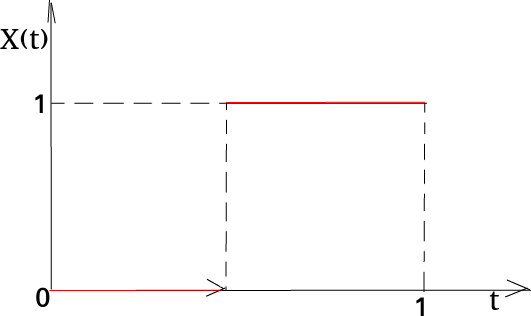
\includegraphics[width=.5\textwidth]{./pictures/2_7.png}
 \caption{Траектория случайного процесса}
 \label{fig:27}
\end{figure}

Случайная величина принимает значения 0 и 1: $X \left( 0 \right) = 0, \, X \left( 1 \right) = 1$,
значит, $X \left( \eta \right) = \eta $.

$$ \varphi_{X \left( \eta \right) } \left( \lambda \right) =
  \varphi_{ \eta } \left( \lambda \right) =
  Me^{i \lambda \eta } =
  \frac{1}{3} \cdot 1 + \frac{2}{3} \cdot e^{i \lambda }.$$

То, что они независимы, тут не важно.

\addcontentsline{toc}{section}{Домашнее задание}
\section*{Домашнее задание}
